\newcommand{\degree}{\ensuremath{^{\circ}}}

\chapter{Kreslenie molekuly}

Po tom čo získame a aplikujeme mapovanie medzi šablonovou a cieľovou molekulou RNA,
ziskame cieľovú molekulu s čiastočnou vizualizáciou, ktorej zvyšok treba dopočitať.

Po operáciach delete ostávajú v molekule prázdne diery, naopak po insertoch potrebujeme
vypočítať, kam umiestnime bázový pár, resp. samotnú bázu, prípadne ešte potrebujeme pre
ňu urobiť miesto. Update vrcholu v strome nerobí žiadne štruktúrne zmeny, zmení sa iba
názov bázy na danom mieste.

Sekundárna štruktúra RNA obsahuje množstvo motivov popisaných na obrázku \ref{obr:RNA_motifs}.
Vo všeobecnosti ale sa každý z týchto motivov skladá zo stemu a loopu.

Stemom budeme ďalej nazývať časť RNA, ktorá zodpovedá vnútornému vrcholu v strome. Loop
budeme označovať listy v RNA strome (lese), nezáleží či je to bulge, interior loop, hairpin
alebo multibranch loop, ako aj ukazuje obrázok \ref{obr:RNA_motifs_stem_loop}.

Stem začína vždy v najvyššom vrchole stromu (v smere ku koreňu), ktorý je zároveň vnútorným
vrcholom a nemá žiadnych súrodencov, ktorý by boli rovnako vnútornými vrcholmi.
To znamená, že do multibranch loop vchádza 1 stem (ten tu konci) a vychádza z nej niekoľko nových stemov.
Naopak pre bulge a interior loop jeden stem vchádza do štruktúry ale pokračuje ďalej.

\begin{figure}[H]
\centering
%trim=left bottom right top
\fbox{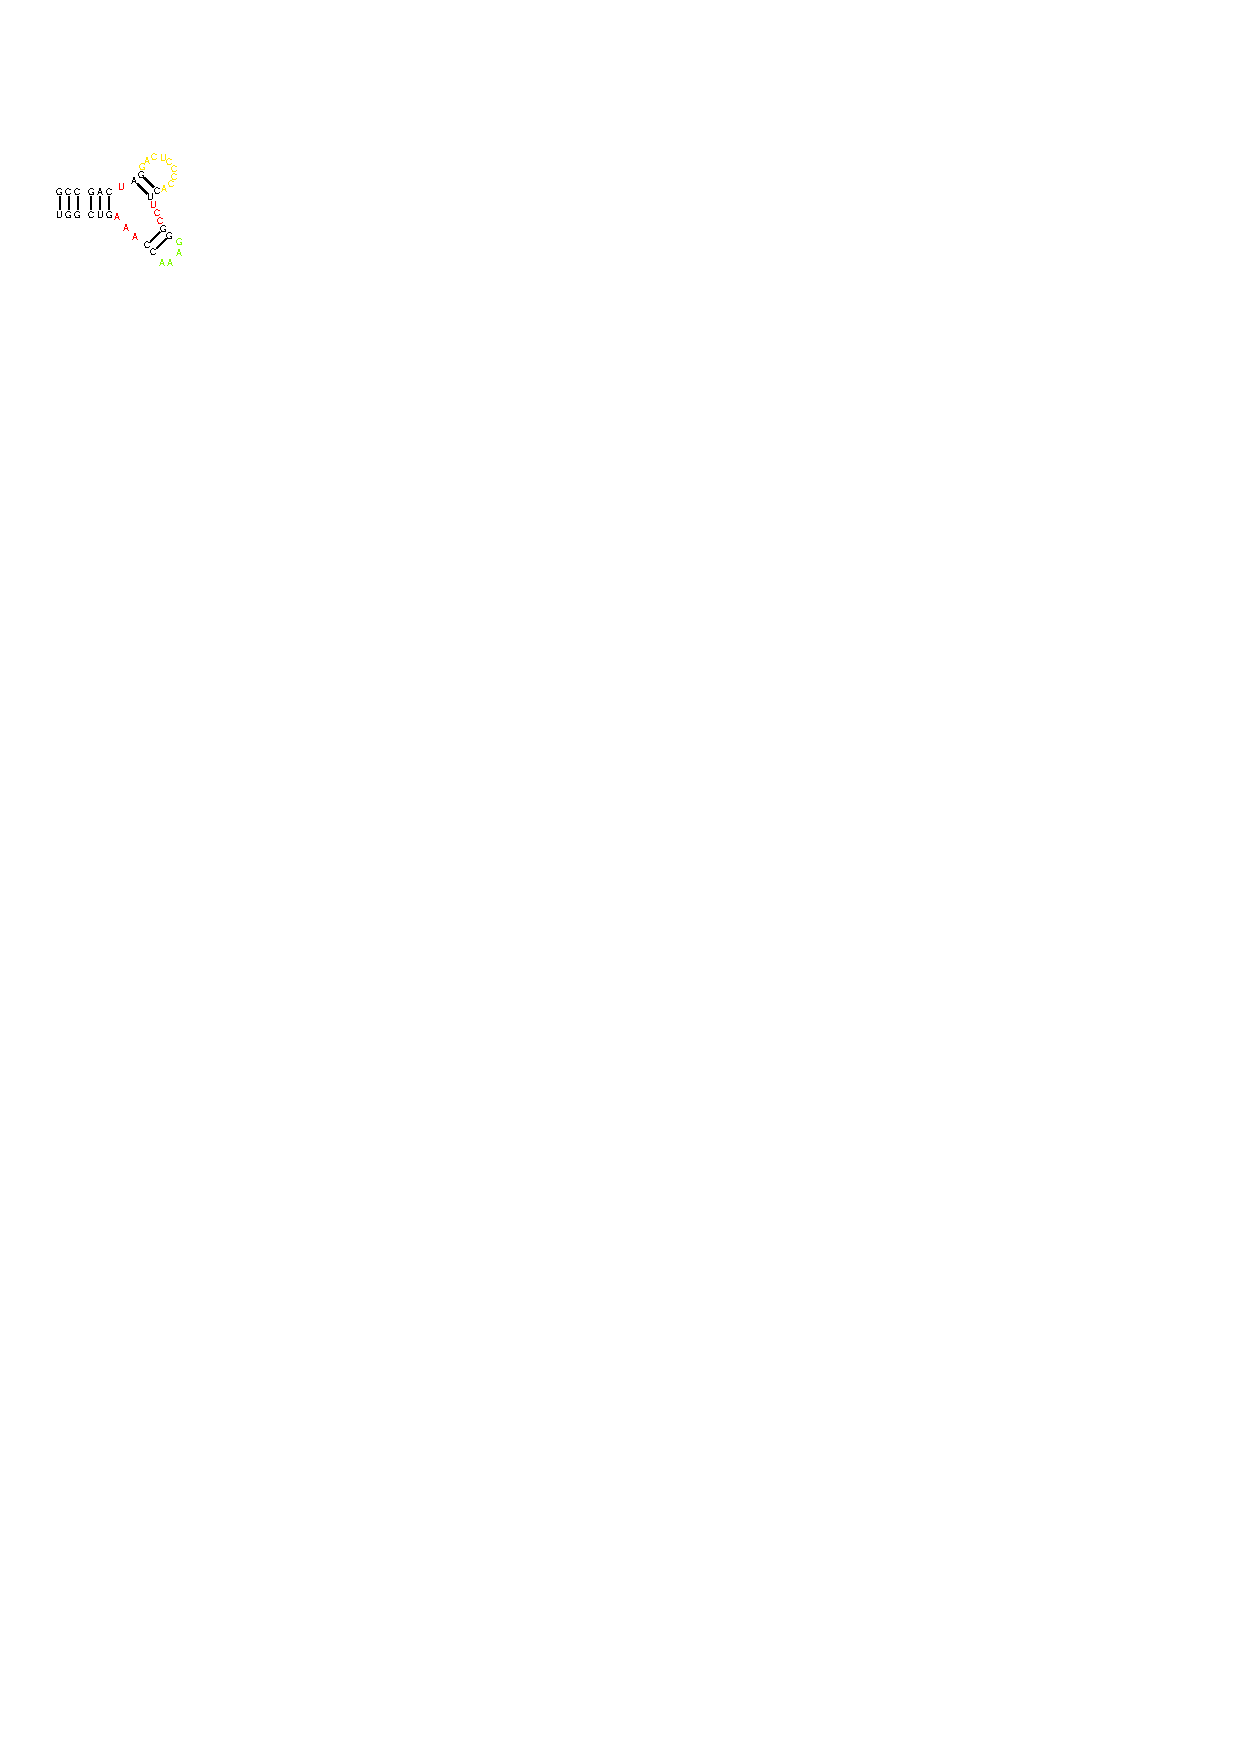
\includegraphics[trim=0.3cm 24.7cm 17cm 2cm]{../img/stem_loop-colored}}
\caption{Rozlisenie stemov a loopov v molekule: cierne su stemy, farebne odlisene su bazy patriace do jednej loopy}
\label{obr:RNA_motifs_stem_loop}
\end{figure}

\section{Štruktúry v RNA}

V článku od \citet{RNA_DRAW} autori popisujú pravidlá vizualizácie sekundárnej štruktúry RNA.

Nakreslenie musí byť rovinné bez krížení, bázy tvoriace rôzne druhy loopov musia ležať na kružniciach
a bázy tvoriace stem majú ležať na priamke.
Ďalším pravidlom je, že vzdialenosť medzi bázami má byť konštantná, či už vzdialenosť medzi bázami jedného páru,
alebo bázami sekvencie.

Ako je ukázane na obrázku \ref{obr:RNA_full}, pravidla niesu niekedy rešpektované. To zťažuje pouzitie obrazka
ako šablony, kedže vo výslednom obrázku chceme všetky tieto pravidlá rešpektovať.

\section{Algoritmus}
Čiastočnej vizualizácie, ktorú dostávame z mapovania sa chceme dotýkať čo najmenej. To znamená,
že všetky zásahy sa snažíme robiť iba v miestach, ktoré boli dotknuté vkladaním alebo mazaním báz.

Jediné výnimky sú normalizácia vzdialensti medzi bázovými pármi a vyrovnávanie stemov.

\subsection{Normalizácia vzdialeností v bázových pároch a vyrovnavanie stemov}

Ako bolo uvedené, stemom rozumieme nevetviacu sa časť stromu tvorenú iba bázovými pármi.

Algoritmus normalizácie vzdialeností medzi vrcholmi bázových párov stojí iba v preiterovaní celého stromu
a ak nejaké párové vrcholy sú od seba príliž vzdialené, priblíži ich k sebe.

Vyrovnávací algoritmus prechádza všetky stemy. Z ich začiatkov vedie priamku, na ktorej majú byť podľa pravidla uložené
všetky stemove vrcholy. Rotáciami a posunutiami podstromov vieme docieliť to, aby vrcholy stemu na tejto priamke ležali.

% TODO obrázok vyrovnávania

\subsection{Operácie na stromoch}

Čitateľa zoznámime s 2 operáciami, ktoré budeme vykonávať na molekule. Tie budeme používať nezávisle
na tom, či vrcholy do stromu vkladáme alebo mažeme.

\begin{algorithm}
  \caption{Rozloženie báz na kružnicu}
  \label{alg:operácia_circle_reinsert}
  \begin{algorithmic}[1]
    \Procedure {rozlozBazy}{Begin, End, Bases}
      \State $n \gets$ veľkosť zoznamu báz $Bases$
      \State $\Gamma \gets$ dostatočne veľká kružnica pre $n$ bodov prechádzajúca bodmi $Begin$ a $End$
      \State $\Pi \gets$ rozdel kruhový obluk kružnice $\Gamma$ od $Begin$ po $End$ na $n$ bodov
      \ForAll{$i$ in 1 .. $n$}
        \State nastav pozíciu bázy $Bases[i]$ na bod $\Pi[i]$
      \EndFor
    \EndProcedure
  \end{algorithmic}
\end{algorithm}

\begin{algorithm}
  \caption{Posunutie podstromu}
  \label{alg:operacia_tree_shift}
  \begin{algorithmic}[1]
    \Procedure {posunPodstrom}{Root, Vector}
      \ForAll {vrchol $V$ v podstrome vrcholu $Root$}
        \If {vrchol $V$ už má určenu pozíciu, t.j. nieje práve vložený}
          \State pripočítaj k pozicií bázy $V$ vektor $Vector$
        \EndIf
      \EndFor
    \EndProcedure
  \end{algorithmic}
\end{algorithm}

Ako sme písali už skôr, všetky loop štruktúry majú byť uložené na kružniciach. K tomu nám pomôže funkcia
\ref{alg:operacia_circle_reinsert}. Tá dostáva na vstupe zoznam báz $Bases$ a dva body v rovine, $Begin$ a $End$.
Týmito bodmi potrebujeme viesť kružnicu, ktorá bude dostatočne veľká, teda aby na ňu všetky bázy zo zoznamu vošli.
Veľkosťou kružnice v tomto prípade myslíme dĺžku kruhového obluku medzi vrcholmi $Begin$ a $End$.

V našom programe používame iteračný algoritmus, ktorý ju pomaly zväčšuje alebo zmenšuje.
Nakoniec buď nájde kružnicu, ktorej veľkosť je optimálna, alebo ani na maximálny počet krokov takú kružnicu nenájde
a tak vráti tu z posledného kroku. Na obrázku \ref{obr:insert_circle_hairpin} vidíme celý algoritmus zväčšovania kružnice.

\begin{figure}
  \begin{subfigure}{0.3\textwidth}
%trim=left bottom right top
    \fbox{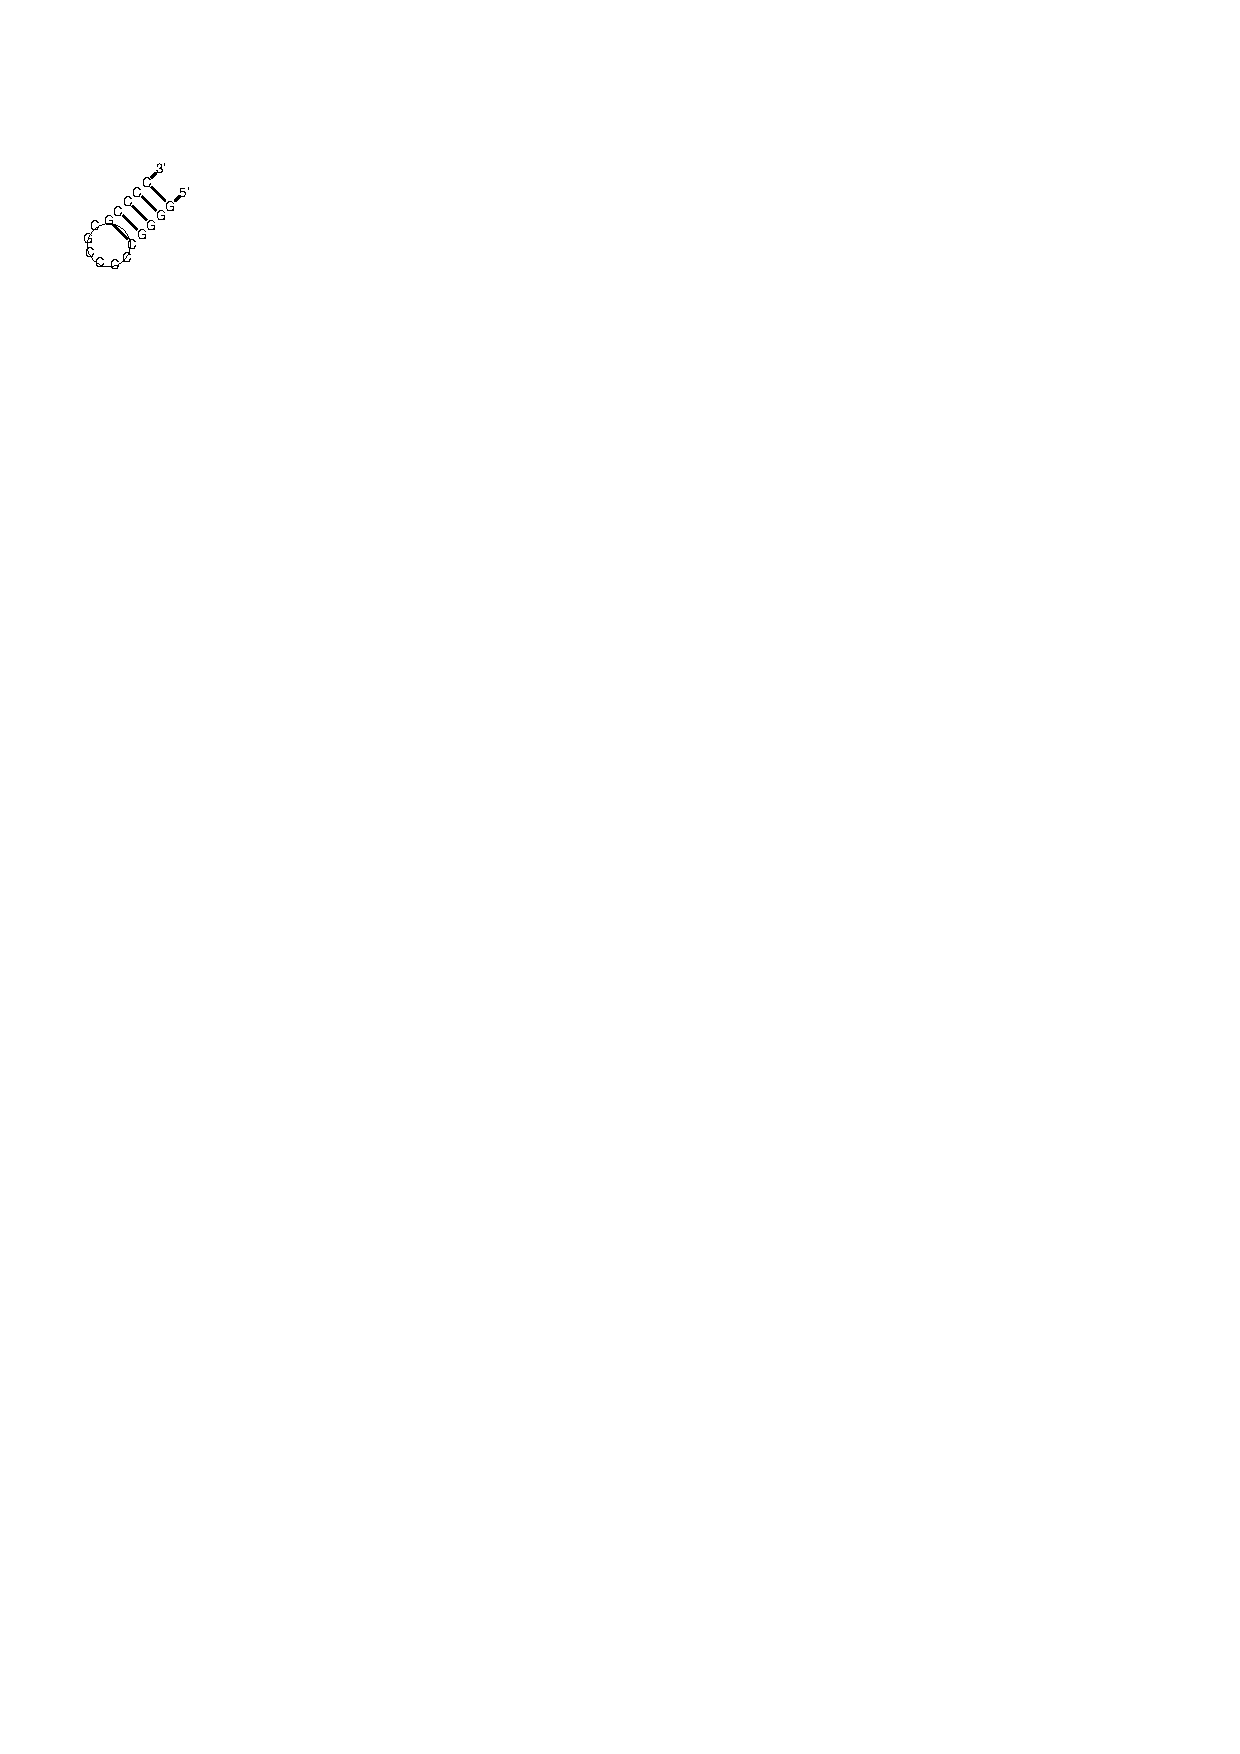
\includegraphics[trim=1cm 24.5cm 17cm 2.5cm]{../img/alg-insert/1/circle-small}}
  \end{subfigure}
  \begin{subfigure}{0.3\textwidth}
    \fbox{\includegraphics[trim=1cm 24.5cm 17cm 2.5cm]{../img/alg-insert/1/circle-big}}
  \end{subfigure}
  \begin{subfigure}{0.3\textwidth}
    \fbox{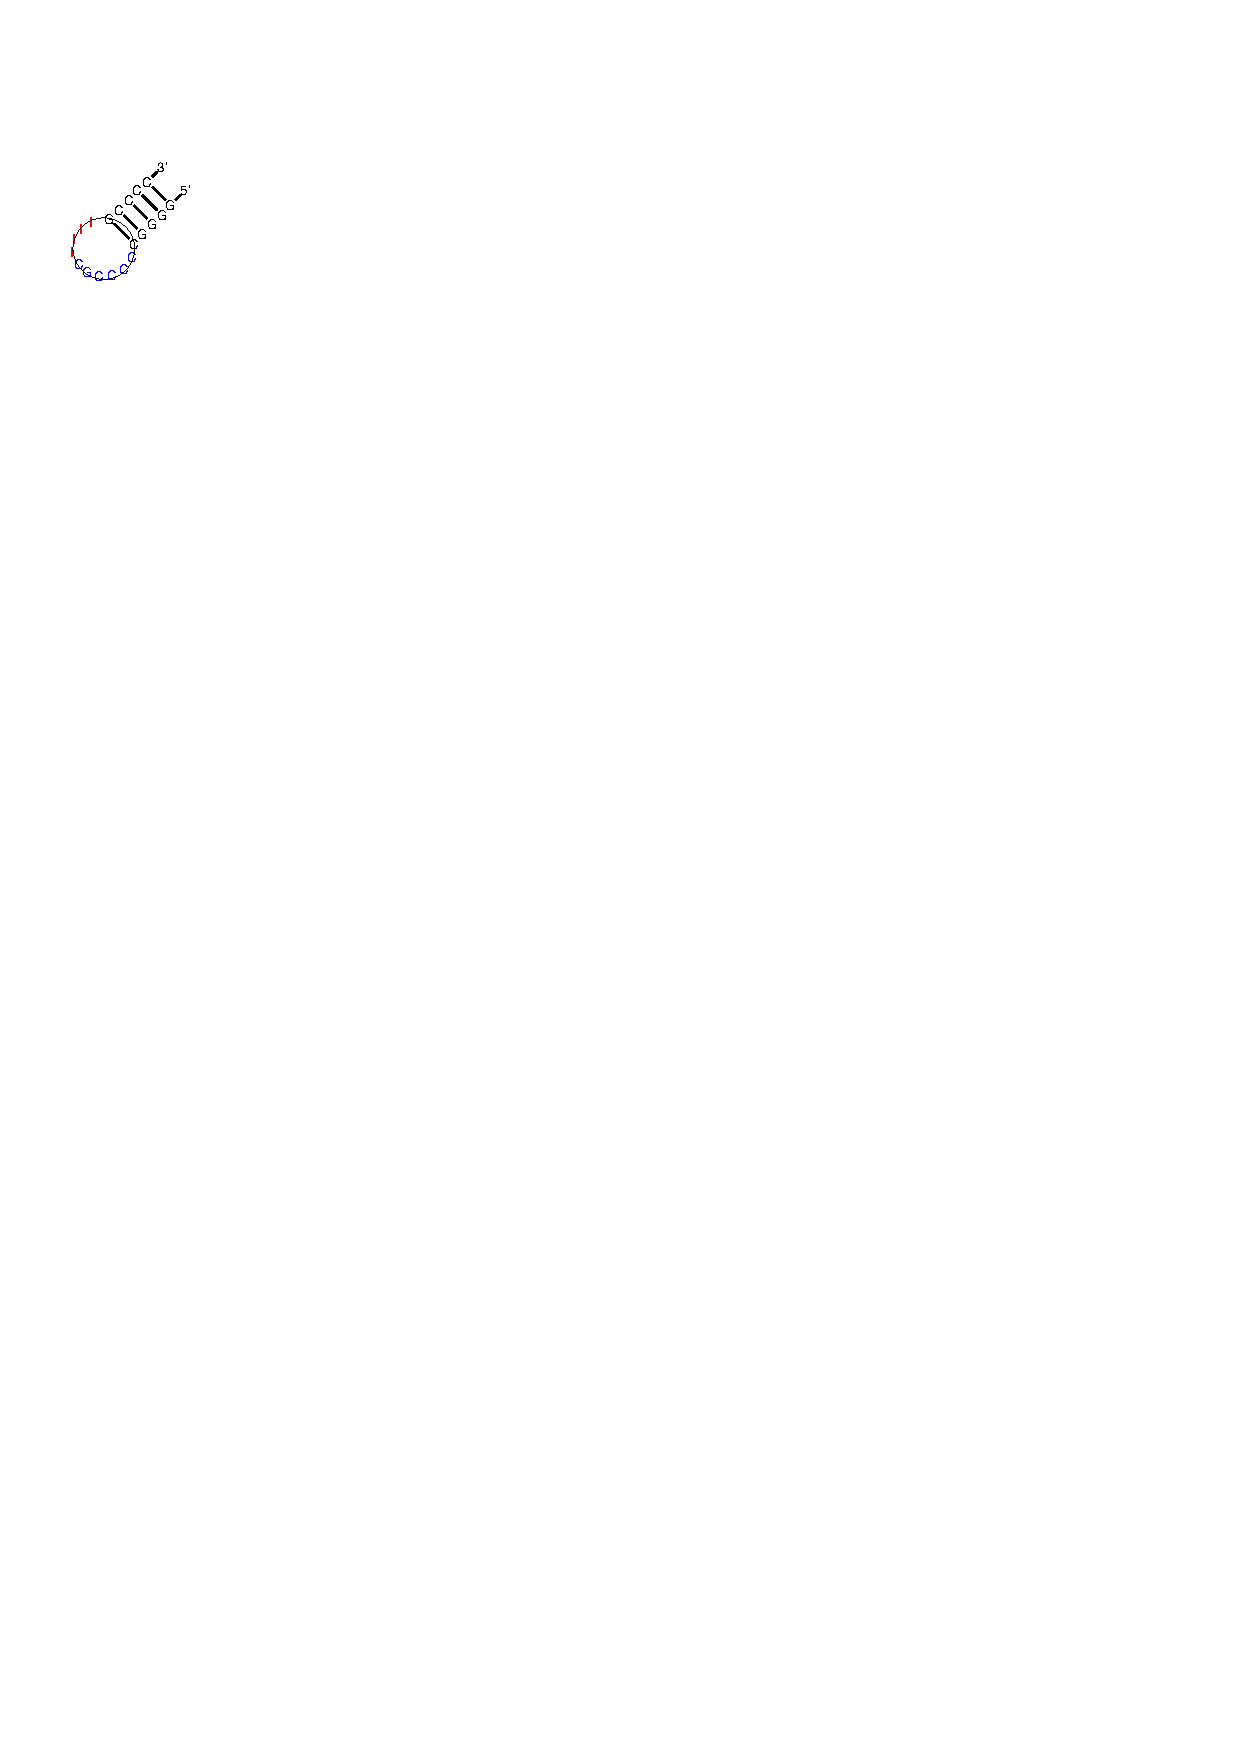
\includegraphics[trim=1cm 24.5cm 17cm 2.5cm]{../img/alg-insert/1/circle-big-end}}
  \end{subfigure}

  \caption{Priklad zvacsovania kruznice a insertu do hairpinu}
  \label{obr:insert_circle_hairpin}
\end{figure}

Operácia v rámci algoritmu \ref{alg:operacia_tree_shift} nám pomôže urobiť miesto na novo vložené bázové páry,
alebo naopak ak sme niečo zmazali, tak dokáže celý podstrom pritiahnuť späť.

\subsection{Vkladanie nového vrcholu do stromu}

Pri vkladaní nového vrcholu do stromu môžu nastať nasledovné možnosti.

Ak vkladáme list do hairpinu, je to jednodúche, potrebujeme iba použiť procedúru z algoritmu \ref{alg:operacia_circle_reinsert}
s parametrami $Begin = $ požicia prvej bázy z bázového páru, $End = $ požičia druhej bázy z páru
a $Bases = $ zoznam všetkých potomkov.

Trochu zložitejšie je to pri vkladaní listu do stemu. V tomto prípade buď už stem obsahoval nejaký loop, alebo vzniká nová.
Najprv potrebujeme upraviť vzdialenosť medzi vrcholmi stemu, teda posunuť celý podstrom aby nám dané bázy vošli.
To vyriešime algoritmom \ref{alg:operacia_tree_shift}. Následne nájdeme kružnicu a bázy na ňu naukladáme.

Vkladanie bázového páru do stemu je jednoduché. Najprv posunieme celý podstrom a urobíme tak miesto pre novú dvojicu
báz, a potom ich uložíme na pozíciu kde by mala patriť. Môže sa stať, že vložením vrcholu do stemu zdedíme niekoľko
listov z predka. V tomto prípade iba použijeme operáciu vloženia vrcholu a updatu loopov pred aj za vloženým vrcholom.

\subsection{Modifikácia multibrach loop}

Modifikácia multibranch loop je zložitejšia ako všetky predchádzajúce prípady. Obrázky sú väčšinou ručné upravené tak,
aby bol čo najkompaktnejší a kvôli tomu sa často nerešpektujú pravidlá o kružnicovom tvare štruktúry.
Kvôli tomu sa snažíme do tejto štruktúry nezasahovať, ak sa to dá.

Prekresleniu celej štruktúry sa môžeme vyhnúť napríklad pri zmene počtu listov medzi jednotlivými vetvami.
Ak je zmena dostatočne malá, môžeme vrcholy roztiahnuť, alebo naopak priblížiť k sebe.

Ak sa jedná o pridanie/odobratie celej vetvy stromu, modifikácií sa nevyhneme. V tom prípade potrebujeme
rozdistribuovať všetky vrcholy patriace do loop na kružnicu. Je to podobný proces ako sa používa iba pre samotné loopy,
ale potrebujeme posúvať celé podstromy a zrotovať ich správnym smerom.

\subsection{Mazanie vrcholu zo stromu}

Mazanie považujeme za inverznú operáciu voči vkladaniu do stromu. Vzhľadom k tomu, používame rovnaké operácie
rozdistribuovania vrcholov v loope, alebo posúvanie podstromu, ktoré sa deje v tomto prípade opačným smerom
k predkovi.

